%% Journal version (Springer Nature template, sn-jnl.cls).  Build: pdflatex, bibtex, pdflatex x2.
%% Numbers come from generated files (experiments/make_*_assets.py); do not edit them by hand.
\documentclass[pdflatex,sn-mathphys-num]{sn-jnl}

\usepackage{graphicx}
\usepackage{multirow}
\usepackage{amsmath,amssymb,amsfonts}
\usepackage{amsthm}
\usepackage{mathrsfs}
\usepackage[title]{appendix}
\usepackage{xcolor}
\usepackage{textcomp}
\usepackage{manyfoot}
\usepackage{booktabs}
\usepackage{tikz}
\usetikzlibrary{arrows.meta,positioning}

\theoremstyle{thmstyleone}
\newtheorem{theorem}{Theorem}
\newtheorem{proposition}[theorem]{Proposition}
\newtheorem{lemma}[theorem]{Lemma}
\newtheorem{corollary}[theorem]{Corollary}
\theoremstyle{thmstylethree}
\newtheorem{definition}{Definition}
\newtheorem{remark}{Remark}

\newcommand{\Cl}{\mathcal C}
\newcommand{\Cay}{\mathrm{Cay}}
\newcommand{\ev}{\mathrm{ev}}
\newcommand{\RXX}{\mathrm{RXX}}\newcommand{\RX}{\mathrm{RX}}\newcommand{\RY}{\mathrm{RY}}\newcommand{\RZ}{\mathrm{RZ}}
\newcommand{\CZ}{\mathrm{CZ}}\newcommand{\SX}{\mathrm{SX}}
\newcommand{\Sp}{\mathrm{Sp}}
\newcommand{\op}[1]{\lVert#1\rVert}
\newcommand{\Dw}{\mathbb D[\omega]}
\newcommand{\Zw}{\mathbb Z[\omega]}
\newcommand{\qcr}{\texttt{qcr}}

\newcommand{\DiamIonThree}{17}
\newcommand{\DiamIonThreePlusOne}{18}
\newcommand{\MeanIonThree}{10.72}
\newcommand{\DiamIbmThree}{19}
\newcommand{\MeanIbmThree}{12.34}
\newcommand{\BFSMinutes}{25}
\newcommand{\OddRelIon}{11}
\newcommand{\OddRelIonMinusOne}{10}
\newcommand{\OddRelIonHalf}{6}
\newcommand{\OddRelIonHalfMinusOne}{5}
\newcommand{\OddRelIbm}{9}
\newcommand{\TwoQThreeDist}{13{,}824/373{,}248/5{,}971{,}968/38{,}486{,}016/42{,}052{,}608/5{,}971{,}968/27{,}648 for $0/\dots/6$ entangling gates}
\newcommand{\TwoQThreeMean}{3.51}
\newcommand{\TwoQThreeMax}{6}
\newcommand{\OptIon}{10.4}
\newcommand{\FaithIon}{47.1}
\newcommand{\EWeightIon}{28.3}
\newcommand{\EWsixteenIon}{10.4}
\newcommand{\FaithIonSec}{51}
\newcommand{\EWeightIonSec}{0.54}
\newcommand{\EWsixteenIonSec}{0.24}
\newcommand{\GapFactorIon}{4.5}
\newcommand{\SpeedupIon}{210}
\newcommand{\WStarIon}{12}
\newcommand{\OptIbm}{12.2}
\newcommand{\FaithIbm}{36.8}
\newcommand{\EWeightIbm}{51.1}
\newcommand{\EWsixteenIbm}{12.2}
\newcommand{\FaithIbmSec}{17}
\newcommand{\EWeightIbmSec}{0.22}
\newcommand{\EWsixteenIbmSec}{0.09}
\newcommand{\GapFactorIbm}{3.0}
\newcommand{\SpeedupIbm}{190}
\newcommand{\WStarIbm}{16}
\newcommand{\GridEightFive}{46.1}
\newcommand{\GridEightInf}{17.9}
\newcommand{\MeanIonTwoEven}{5.90}
\newcommand{\MeanIonTwoOdd}{5.88}
\newcommand{\BetaTwo}{0.937}
\newcommand{\LMixTwo}{133}
\newcommand{\MixLThree}{100}
\newcommand{\LBFourIon}{11.1}
\newcommand{\LBFourIbm}{12.9}
\newcommand{\LBThreeCheck}{7.9}
\newcommand{\CWFourIon}{56.7}
\newcommand{\CWFourIonTwoQ}{27.6}
\newcommand{\CWFourSec}{5.6}
\newcommand{\EWFourSec}{0.8}
\newcommand{\FaithFourSec}{65}
\newcommand{\EWFourIon}{110.3}
\newcommand{\EWFourIonTwoQ}{44.2}
\newcommand{\FaithFourIon}{78.8}
\newcommand{\FaithFourIonTwoQ}{33.3}
\newcommand{\QFourIon}{164.9}
\newcommand{\QFourIonTwoQ}{47.3}
\newcommand{\FourImprovementIon}{49\%}
\newcommand{\QThreeIon}{127.2}
\newcommand{\CWFourIbm}{59.1}
\newcommand{\CWFourIbmTwoQ}{27.1}
\newcommand{\EWFourIbm}{130.9}
\newcommand{\EWFourIbmTwoQ}{47.1}
\newcommand{\FaithFourIbm}{76.0}
\newcommand{\FaithFourIbmTwoQ}{32.4}
\newcommand{\QFourIbm}{140.9}
\newcommand{\QFourIbmTwoQ}{47.3}
\newcommand{\FourImprovementIbm}{45\%}
\newcommand{\QThreeIbm}{104.0}
\newcommand{\GapFindings}{\paragraph{Findings.} (1) On its own benchmark the original method finishes \GapFactorIon$\times$ (ion trap) and
\GapFactorIbm$\times$ (IBM-style) above the exact optimum. Our faithful port reproduces the paper's single-circuit number
(\FaithIon\ vs.\ 45 gates), so the gap is a property of the method, not of our implementation. (2) EW-$w$ reaches the
\emph{proven} optimum on all 20 circuits once $w\ge\WStarIon$ (ion trap) or $w\ge\WStarIbm$ (IBM-style), in a fraction of a second.
This is the cascade of Prop.~\ref{prop:cascade}: the transition is sharp, between $w=8$ and $w=12$ (ion trap) or $w=16$ (IBM-style). (3) The grid (Fig.~\ref{fig:grid})
shows that the \emph{database radius}, not the window or the search strategy, is the binding constraint. At $r=5$, enlarging the
window from 8 to 16 lowers the mean excess only from 46 to 43 gates. At $w=8$, raising $r$ from 5 to $\infty$ lowers it from 46 to 18,
and for $w\ge12$ with $r\ge8$ the excess is at most 2 gates (ion trap; IBM-style: from 72 to $\le$\,8). Theorem~\ref{thm:exact} predicts
both requirements: windows long enough \emph{and} a database deep enough. The original method is limited by the second.
}
\newcommand{\FourFindings}{\paragraph{Findings.} (1) \emph{Convexity matters more than anything else at $n\ge4$.} With the same exact 3-qubit
oracle, contiguous windows (EW-16) give \EWFourIon\ (ion trap) and \EWFourIbm\ (IBM-style) gates, no better than the
published method. With DAG-convex windows (CW-24) the same oracle gives \CWFourIon\ and \CWFourIbm\ gates, i.e.\
\FourImprovementIon\ and \FourImprovementIbm\ fewer than the published results, in about \CWFourSec\,s per circuit. (2)
Two-qubit counts drop from 43 (published) to \CWFourIonTwoQ\ RXX and \CWFourIbmTwoQ\ CZ, on par with BQSKit L4 for the ion trap (28) and
below it for the IBM-style set (37), although CW optimises total length, not two-qubit count. (3) The certified lower bounds
(\LBFourIon, \LBFourIbm) leave a gap of at most a factor $\approx5$. Closing it, either by tightening the bound (deeper spheres,
meet-in-the-middle) or by better upper bounds (4-qubit oracles via symmetry reduction), is an open problem that our framework
makes precise.
}

% generated by experiments/make_general_assets.py -- do not edit
\newcommand{\HwCircuits}{60}
\newcommand{\HwCompared}{58}
\newcommand{\HeronFromLThreeBetter}{9}
\newcommand{\HeronFromLThreeEqual}{49}
\newcommand{\HeronFromLThreeWorse}{0}
\newcommand{\HeronFromLThreeTotalUp}{1}
\newcommand{\HeronFromLThreeSuccDown}{0}
\newcommand{\HeronEspLOneOverLThree}{1.11}
\newcommand{\HeronEspOursOverLOne}{1.09}
\newcommand{\HeronLThreeRz}{5297}
\newcommand{\HeronLThreePulse}{7218}
\newcommand{\HeronLThreeTwoq}{2889}
\newcommand{\HeronFromLThreeRz}{4436}
\newcommand{\HeronFromLThreePulse}{6139}
\newcommand{\HeronFromLThreeTwoq}{2830}
\newcommand{\HeronMaxQubits}{12}
\newcommand{\HeronMaxInput}{1008}
\newcommand{\HeronRuns}{360}
\newcommand{\HeronUnverified}{5}
\newcommand{\HeronMaxExactErr}{1.9\cdot10^{-11}}
\newcommand{\HeronMaxStateErr}{2\cdot10^{-12}}
\newcommand{\HeronMaxApproxErr}{6.4\cdot10^{-4}}
\newcommand{\HeronApproxWithinBound}{59}
\newcommand{\HeronAllLegal}{60}
\newcommand{\HeronStateEmpty}{5}
\newcommand{\HeronPhaseGadgetGates}{240}
\newcommand{\HeronMedianSec}{10.4}
\newcommand{\HeronMaxSec}{180}
\newcommand{\HeronTvdCircuits}{49}
\newcommand{\HeronTvdLThree}{0.137}
\newcommand{\HeronTvdLOne}{0.115}
\newcommand{\HeronTvdCount}{0.096}
\newcommand{\HeronTvdWTwo}{0.088}
\newcommand{\HeronTvdCal}{0.088}
\newcommand{\HeronCalBeatsLThree}{39}
\newcommand{\HeronCalBeatsCount}{41}
\newcommand{\IonFromLThreeBetter}{1}
\newcommand{\IonFromLThreeEqual}{57}
\newcommand{\IonFromLThreeWorse}{0}
\newcommand{\IonFromLThreeTotalUp}{28}
\newcommand{\IonFromLThreeSuccDown}{0}
\newcommand{\IonEspLOneOverLThree}{0.99}
\newcommand{\IonEspOursOverLOne}{1.02}
\newcommand{\IonLThreeRz}{2223}
\newcommand{\IonLThreePulse}{3824}
\newcommand{\IonLThreeTwoq}{1378}
\newcommand{\IonFromLThreeRz}{3622}
\newcommand{\IonFromLThreePulse}{2422}
\newcommand{\IonFromLThreeTwoq}{1376}
\newcommand{\IonMaxQubits}{12}
\newcommand{\IonMaxInput}{1008}
\newcommand{\IonRuns}{360}
\newcommand{\IonUnverified}{0}
\newcommand{\IonMaxExactErr}{8.2\cdot10^{-11}}
\newcommand{\IonMaxStateErr}{6\cdot10^{-12}}
\newcommand{\IonMaxApproxErr}{1.4\cdot10^{-4}}
\newcommand{\IonApproxWithinBound}{60}
\newcommand{\IonAllLegal}{60}
\newcommand{\IonStateEmpty}{7}
\newcommand{\IonPhaseGadgetGates}{52}
\newcommand{\IonMedianSec}{3.0}
\newcommand{\IonMaxSec}{96}
\newcommand{\IonTvdCircuits}{49}
\newcommand{\IonTvdLThree}{0.0091}
\newcommand{\IonTvdLOne}{0.0157}
\newcommand{\IonTvdCount}{0.0092}
\newcommand{\IonTvdWTwo}{0.0084}
\newcommand{\IonTvdCal}{0.0084}
\newcommand{\IonCalBeatsLThree}{29}
\newcommand{\IonCalBeatsCount}{26}
\newcommand{\PfOneLThreeTwoq}{0}
\newcommand{\PfOneOursTwoq}{139}
\newcommand{\PfOneLOneTwoq}{153}
\newcommand{\PfTwoLThreeTwoq}{0}
\newcommand{\PfTwoOursTwoq}{298}
\newcommand{\PfTwoLOneTwoq}{300}
\newcommand{\PaperBenchN}{250}
\newcommand{\PaperBenchOk}{250}
\newcommand{\TThreeGen}{10.8}
\newcommand{\TThreeGenSec}{2.6}
\newcommand{\TThreeN}{20}
\newcommand{\TThreePaper}{47.1}
\newcommand{\TThreePaperN}{20}
\newcommand{\TThreeGenOverPaper}{0.25}
\newcommand{\TThreeLThree}{127.2}
\newcommand{\TThreeCliff}{--}
\newcommand{\TThreeOpt}{10.4}
\newcommand{\TThreeAtOpt}{17}
\newcommand{\TFourGen}{12.5}
\newcommand{\TFourGenSec}{2.8}
\newcommand{\TFourN}{20}
\newcommand{\TFourPaper}{36.8}
\newcommand{\TFourPaperN}{20}
\newcommand{\TFourGenOverPaper}{0.42}
\newcommand{\TFourLThree}{104.0}
\newcommand{\TFourCliff}{--}
\newcommand{\TFourOpt}{12.2}
\newcommand{\TFourAtOpt}{18}
\newcommand{\NjpIonGen}{46.1}
\newcommand{\NjpIonGenSec}{7.7}
\newcommand{\NjpIonN}{100}
\newcommand{\NjpIonPaper}{78.8}
\newcommand{\NjpIonPaperN}{30}
\newcommand{\NjpIonGenOverPaper}{0.57}
\newcommand{\NjpIonLThree}{164.9}
\newcommand{\NjpIonCliff}{45.6}
\newcommand{\NjpIonOpt}{--}
\newcommand{\NjpIbmGen}{51.4}
\newcommand{\NjpIbmGenSec}{8.5}
\newcommand{\NjpIbmN}{100}
\newcommand{\NjpIbmPaper}{76.0}
\newcommand{\NjpIbmPaperN}{30}
\newcommand{\NjpIbmGenOverPaper}{0.70}
\newcommand{\NjpIbmLThree}{140.9}
\newcommand{\NjpIbmCliff}{49.3}
\newcommand{\NjpIbmOpt}{--}
\newcommand{\TFiveGen}{327.7}
\newcommand{\TFiveGenSec}{8.9}
\newcommand{\TFiveN}{10}
\newcommand{\TFivePaper}{335.9}
\newcommand{\TFivePaperN}{10}
\newcommand{\TFiveGenOverPaper}{0.98}
\newcommand{\TFiveLThree}{332.1}
\newcommand{\TFiveCliff}{324.6}
\newcommand{\TFiveOpt}{--}

% generated by experiments/make_general_assets.py -- do not edit
\newcommand{\HwRows}{%
TKET (FullPeepholeOptimise on L1) & \(\times\)1.02 & \(\times\)1.71 & \(\times\)1.16 && \(\times\)1.27 & \(\times\)1.79 & \(\times\)0.992\\
\midrule
ours, exact, from L1 & \(\times\)1.00 & \(\times\)0.84 & \(\times\)1.21 && \(\times\)0.95 & \(\times\)0.76 & \(\times\)1.002\\
ours, exact, from L3 & \(\times\)0.98 & \(\times\)0.87 & \(\times\)1.03 && \(\times\)1.00 & \(\times\)1.00 & \(\times\)1.001\\
ours, approximate ($\varepsilon=10^{-3}$), from L1 & \(\times\)1.01 & \(\times\)0.84 & \(\times\)1.21 && \(\times\)0.95 & \(\times\)0.75 & \(\times\)1.002\\
ours, state/measurement-aware, from L1 & \(\times\)0.77 & \(\times\)0.61 & \(\times\)1.28 && \(\times\)0.62 & \(\times\)0.50 & \(\times\)1.010\\
}

% generated by experiments/make_new_assets.py -- do not edit
\newcommand{\CTRadius}{5}
\newcommand{\CTBallSize}{698{,}512}
\newcommand{\CTBallLevels}{1, 34, 569, 6{,}744, 67{,}664, 623{,}500}
\newcommand{\CTBallMinutes}{8}
\newcommand{\CTCertified}{9}
\newcommand{\CTRandN}{100}
\newcommand{\CTRandCert}{99}
\newcommand{\CTRandGenAtOpt}{99/99}
\newcommand{\CTRandOrigAtOpt}{81/99}
\newcommand{\CTPlantN}{41}
\newcommand{\CTPlantGenAtOpt}{41}
\newcommand{\CTPlantOrigAtOpt}{40}
\newcommand{\CTPlantInputMean}{90.3}
\newcommand{\CTPlantOptMean}{6.1}
\newcommand{\CTPlantGenMean}{6.1}
\newcommand{\CTPlantOrigMean}{6.1}
\newcommand{\CTPlantQiskitMean}{7.7}
\newcommand{\LayN}{8}
\newcommand{\LayEspLThree}{0.63}
\newcommand{\LayEspNAOurs}{1.01}
\newcommand{\LayEspRel}{1.14}
\newcommand{\LayEspJoint}{1.14}
\newcommand{\LayTwoqLThree}{493}
\newcommand{\LayTwoqNA}{493}
\newcommand{\LayTwoqNAOurs}{485}
\newcommand{\LayTwoqRel}{485}
\newcommand{\LayTwoqJoint}{471}
\newcommand{\LayTvdN}{5}
\newcommand{\LayTvdLThree}{0.569}
\newcommand{\LayTvdNA}{0.332}
\newcommand{\LayTvdNAOurs}{0.325}
\newcommand{\LayTvdRel}{0.225}
\newcommand{\LayTvdJoint}{0.222}
\newcommand{\LayJointBeatsNA}{5}
\newcommand{\LayJointNAShare}{50\%}
\newcommand{\LayMaxErr}{2.5e-12}


\usepackage{xr}\externaldocument{extension_paper}

\begin{document}
\title{Figures and tables}
\author{\fnm{Arnav} \sur{Kapoor}}
\affil{\orgname{IISER Bhopal}}
\abstract{All figures and tables of ``Exact, hardware-aware local rewriting of quantum circuits, with certified ground
truth'', regenerated from the results in this repository. Values shown as ?? come from runs that have not finished.}
\maketitle
\addcontentsline{toc}{section}{Equivalence as a group action}\markboth{Equivalence as a group action}{}

\begin{center}\large\bfseries Equivalence as a group action\end{center}

\begin{table}[h!]
\caption{Equivalence notions as group actions. Notions compose. For example, output-aware equivalence modulo chip symmetries
uses row-normalised matrices minimised over the automorphism group.}\label{tab:actions}
\begin{tabular*}{\textwidth}{@{\extracolsep\fill}llll}
\toprule
notion & $U\sim V$ iff & group acting & canonical key\\
\midrule
exact & $V=U$ & trivial & $U$\\
up to phase~\cite{rosenhahn2025} & $V=e^{i\varphi}U$ & $U(1)$ & phase-normalised $U$\\
input-aware & $V|0\rangle=e^{i\varphi}U|0\rangle$ & stabiliser of $|0\rangle$ & phase-normalised $U|0\rangle$\\
output-aware & $V=DU$, $D$ diagonal & diagonal unitaries & rows phase-normalised\\
symmetry & $V=PUP^\dagger$ & coupling-graph automorphisms & minimum over the orbit\\
approximate & $\op{U-V}\le\varepsilon$ & (a tolerance) & exact key, verified distance\\
\botrule
\end{tabular*}
\end{table}

\clearpage

\addcontentsline{toc}{section}{The optimiser}\markboth{The optimiser}{}

\begin{center}\large\bfseries The optimiser\end{center}

\begin{table}[h!]
\caption{Hashed databases of the general optimiser (classes per equivalence notion).}\label{tab:dbs}
\begin{tabular*}{\textwidth}{@{\extracolsep\fill}lllrrr}
\toprule
device & topology & notion & depth & classes & build time\\
\midrule
Heron & line & up to phase & 9 & 6.31M & 6 min\\
Heron & line & output-aware & 10 & 0.34M & $<$1 min\\
Heron & line & input-aware & 14 & 1.41M & $<$1 min\\
ion & triangle & up to phase & 6 & 28.4M & 38 min\\
ion & triangle & output-aware & 6 & 7.36M & 27 min\\
ion & triangle & input-aware & 7 & 31.6M & 23 min\\
paper ion ($\pm\frac\pi2$) & triangle & up to phase & 9 & 2.93M & 7 min\\
paper IBM ($\pm\frac\pi2$) & triangle & up to phase & 10 & 1.84M & 2 min\\
\botrule
\end{tabular*}
\end{table}

\clearpage

\addcontentsline{toc}{section}{Certified ground truth}\markboth{Certified ground truth}{}

\begin{center}\large\bfseries Certified ground truth\end{center}

\begin{table}[h!]
\caption{Exact Cayley-graph data of the Clifford groups generated by the alphabets of~\cite{rosenhahn2025}.}\label{tab:growth}
\begin{tabular*}{\textwidth}{@{\extracolsep\fill}lrrrrr}
\toprule
alphabet & $n$ & $|\Gamma|$ & $|G|$ & diameter & mean $|g|$ (uniform)\\
\midrule
ion & 2 & 14 & 11,520 & 10 & 5.89\\
IBM-style & 2 & 9 & 11,520 & 11 & 6.92\\
ion & 3 & 24 & 92,897,280 & \DiamIonThree & \MeanIonThree\\
IBM-style & 3 & 15 & 92,897,280 & \DiamIbmThree & \MeanIbmThree\\
\botrule
\end{tabular*}
\end{table}

\clearpage

\begin{figure}[h!]
\centering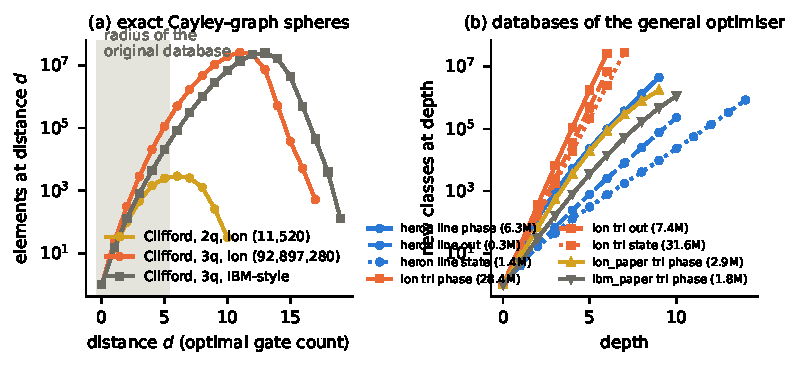
\includegraphics[width=\textwidth]{figs/fig_growth.pdf}
\caption{(a) Sphere sizes of the exact Cayley graphs used as ground truth. The shaded band is the radius of the original
database. The Clifford+T sphere sizes keep growing roughly tenfold per level, since the group is infinite. (b) Level sizes of the
general optimiser's databases (keys per depth, one curve per device, topology and equivalence notion).}\label{fig:growth}
\end{figure}

\clearpage

\begin{figure}[h!]
\centering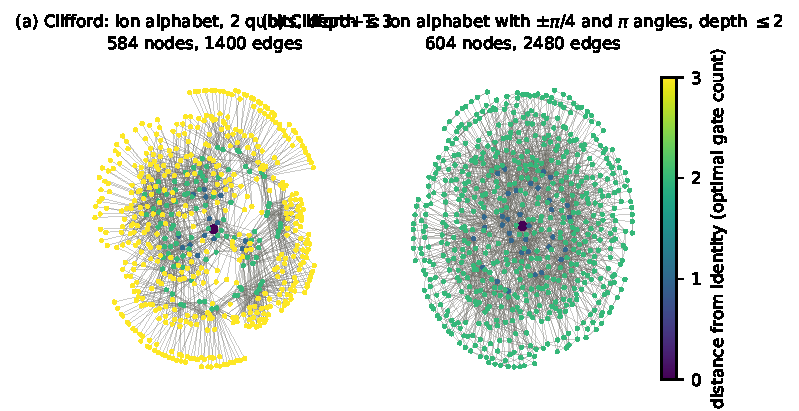
\includegraphics[width=\textwidth]{figs/fig_compute_graph.pdf}
\caption{Compute graphs of comparable size, nodes coloured by exact distance from the identity. (a) Two-qubit Clifford
group, ion alphabet, depth $\le3$. Many short words coincide, and the ball closes up. (b) Two-qubit Clifford+T, depth
$\le2$. Almost every word is new.}\label{fig:cg}
\end{figure}

\clearpage

\addcontentsline{toc}{section}{Experiments}\markboth{Experiments}{}

\begin{center}\large\bfseries Experiments\end{center}

\begin{table}[h!]
\caption{Mean gate counts on the original benchmarks. $^*$Original and Qiskit at 4 qubits use the first 30 circuits.
Qiskit is level 3, orig.\ is the original method, and Cliff.\ CW uses adaptive commutation-aware windows with the exact
Clifford tables (Appendix~\ref{app:cliff}), which the general optimiser does not use. Optimum is the proven optimum or a
certified lower bound, and \#opt.\ counts the circuits on which the general optimiser is optimal. All \PaperBenchOk/\PaperBenchN\ outputs verified and native.}\label{tab:paperbench}
\small
\begin{tabular*}{\textwidth}{@{\extracolsep\fill}lcccccc}
\toprule
setting & Qiskit & orig. & Cliff.\ CW & general & optimum & \#opt.\\
\midrule
T3, ion, 3q & \QThreeIon & \TThreePaper & -- & \TThreeGen & \TThreeOpt & \TThreeAtOpt/20\\
T4, IBM-style, 3q & \QThreeIbm & \TFourPaper & -- & \TFourGen & \TFourOpt & \TFourAtOpt/20\\
journal, ion, 4q & \QFourIon$^*$ & \NjpIonPaper$^*$ & \NjpIonCliff & \NjpIonGen & $\ge$\LBFourIon & --\\
journal, IBM-style, 4q & \QFourIbm$^*$ & \NjpIbmPaper$^*$ & \NjpIbmCliff & \NjpIbmGen & $\ge$\LBFourIbm & --\\
T5, IBM-style, 15q & \TFiveLThree & \TFivePaper & \TFiveCliff & \TFiveGen & -- & --\\
\botrule
\end{tabular*}
\end{table}

\clearpage

\begin{figure}[h!]
\centering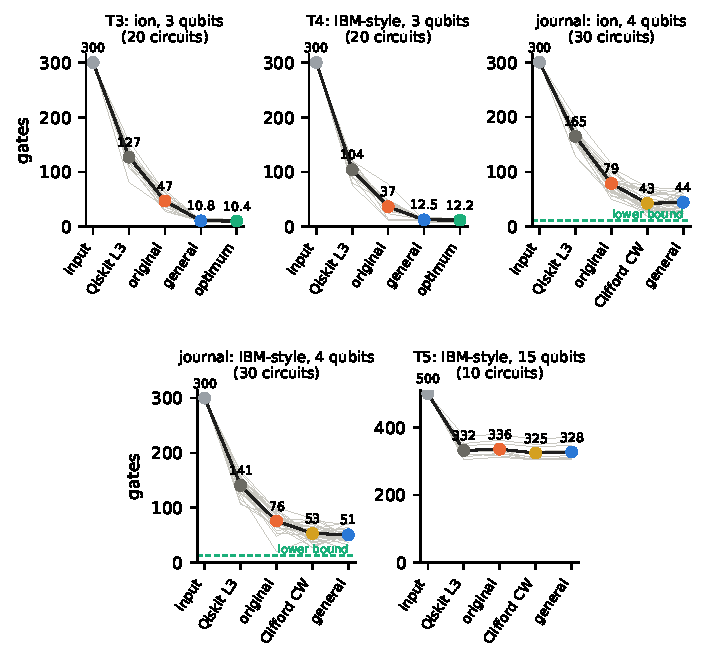
\includegraphics[width=\textwidth]{figs/fig_paper_flow.pdf}
\caption{From the input to the output of every method on the original benchmarks. Grey lines are individual circuits (paired by seed) and
the black line is the mean. The dashed line at 4 qubits is the certified lower bound of Proposition~\ref{prop:count}.}\label{fig:paperflow}
\end{figure}

\clearpage

\begin{figure}[h!]
\centering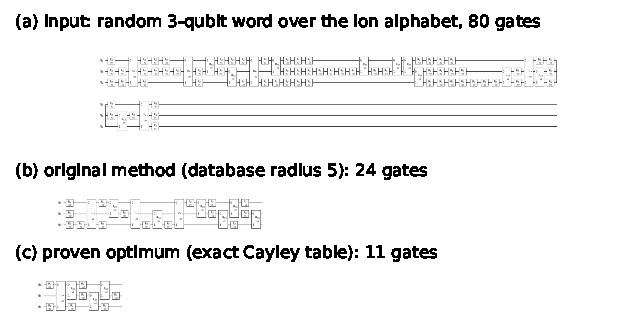
\includegraphics[width=\textwidth]{figs/fig_example_paper.pdf}
\caption{A random 3-qubit word over the ion alphabet (a), the output of the original method (b) and the proven optimum from the
exact Cayley table (c).}\label{fig:expaper}
\end{figure}

\clearpage

\begin{figure}[h!]
\centering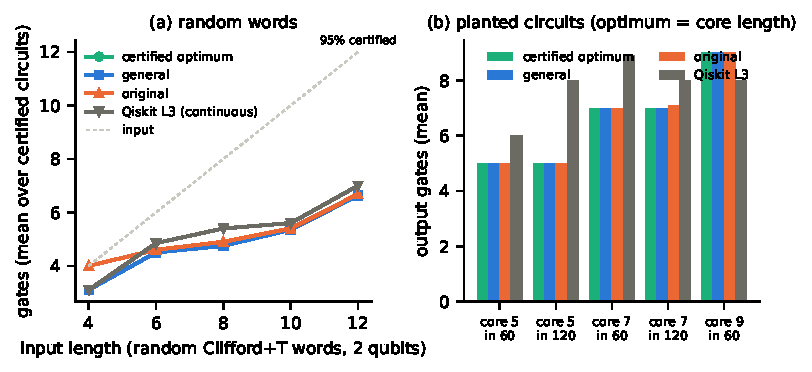
\includegraphics[width=\textwidth]{figs/fig_cliffordt.pdf}
\caption{Clifford+T, two qubits. (a) Random words, mean output length over circuits whose optimum is certified (annotations give
the fraction certified). (b) Planted circuits, a core of the stated length hidden in 60 or 120 gates.}\label{fig:ct}
\end{figure}

\clearpage

\begin{figure}[h!]
\centering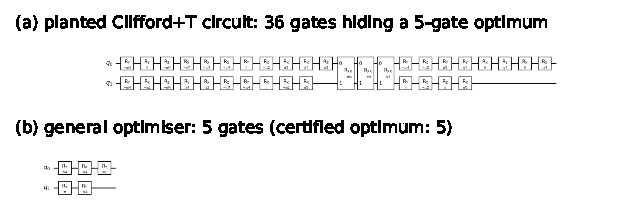
\includegraphics[width=\textwidth]{figs/fig_example_cliffordt.pdf}
\caption{A planted Clifford+T circuit (a) and the output of the general optimiser (b), which equals the certified optimum.}
\label{fig:exct}
\end{figure}

\clearpage

\begin{table}[h!]
\caption{Relative to Qiskit level 3 (\HwCompared\ circuits per device). Count columns are ratios of summed counts, and ESP
is the geometric mean of per-circuit ratios. BQSKit outputs are approximate. Nam pf1\_10/pf2\_10 are excluded because Qiskit level 3 drops their $\sim10^{-7}$\,rad rotations
(approximately, not exactly).}\label{tab:hw}
\begin{tabular*}{\textwidth}{@{\extracolsep\fill}lccc c ccc}
\toprule
& \multicolumn{3}{c}{IBM Heron} && \multicolumn{3}{c}{trapped ion}\\\cmidrule{2-4}\cmidrule{6-8}
pipeline & 2q & all & ESP && 2q & all & ESP\\
\midrule
\HwRows
\botrule
\end{tabular*}
\end{table}

\clearpage

\begin{figure}[h!]
\centering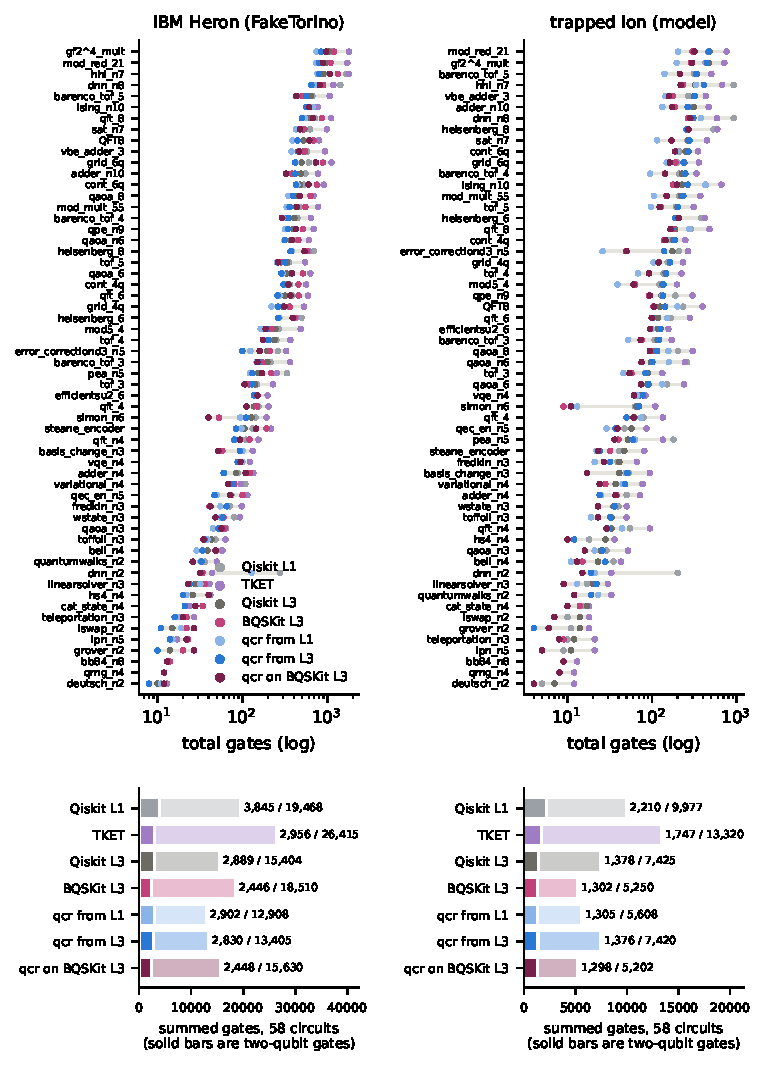
\includegraphics[width=\textwidth]{figs/fig_hw_flow.pdf}
\caption{Hardware suite, from the level-1 compilation to every pipeline's output. The top panel shows total gates per circuit (sorted by
the level-3 count), the bottom panel the sums over all circuits, with two-qubit gates as solid bars.}\label{fig:hwflow}
\end{figure}

\clearpage

\begin{figure}[h!]
\centering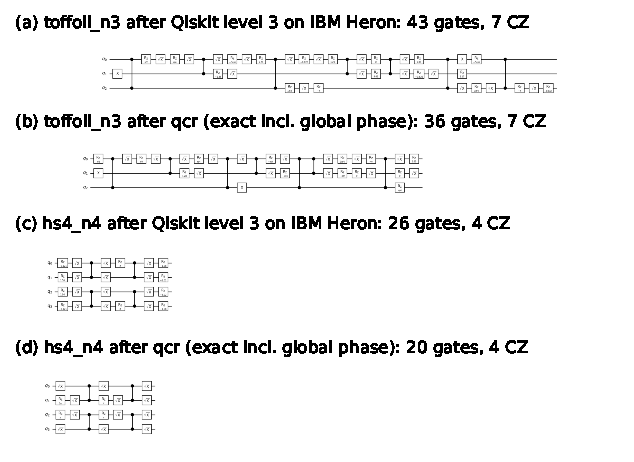
\includegraphics[width=\textwidth]{figs/fig_example_heron.pdf}
\caption{Two QASMBench circuits after Qiskit level 3 on IBM Heron (a, c) and after \qcr\ (b, d). The outputs are equal
including global phase.}\label{fig:exheron}
\end{figure}

\clearpage

\begin{table}[h!]
\caption{Mean noisy-simulation TVD by objective (lower is better).}\label{tab:tvd}
\begin{tabular*}{\textwidth}{@{\extracolsep\fill}lccccc}
\toprule
& Qiskit L1 & Qiskit L3 & ours, count & ours, $w2$ & ours, calibrated\\
\midrule
Heron & \HeronTvdLOne & \HeronTvdLThree & \HeronTvdCount & \HeronTvdWTwo & \HeronTvdCal\\
ion & \IonTvdLOne & \IonTvdLThree & \IonTvdCount & \IonTvdWTwo & \IonTvdCal\\
\botrule
\end{tabular*}
\end{table}

\clearpage

\begin{figure}[h!]
\centering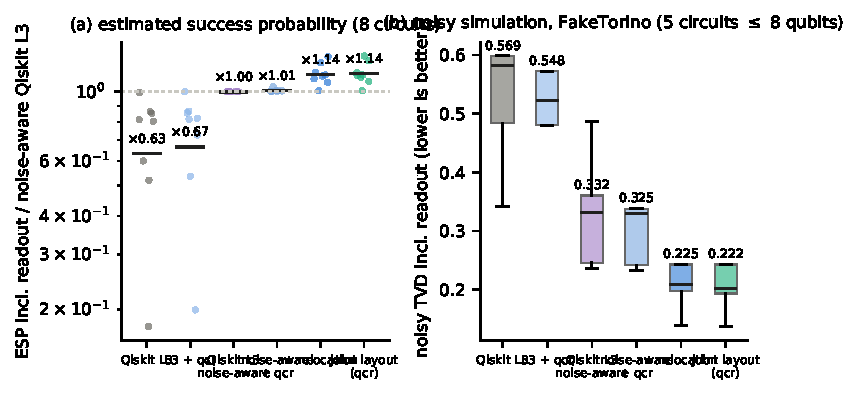
\includegraphics[width=\textwidth]{figs/fig_layout.pdf}
\caption{Layout-aware rewriting on IBM Heron (FakeTorino). (a) ESP including readout relative to Qiskit's noise-aware level 3
(dots are circuits, bars and labels are geometric means). (b) Exact noisy TVD including readout for circuits with at most eight
active qubits (labels: means).}\label{fig:layout}
\end{figure}

\clearpage

\begin{table}[h!]
\caption{Layout-aware rewriting on IBM Heron. ESP includes readout, and ratios are geometric means relative to Qiskit's
noise-aware level 3. TVD: mean exact noisy TVD including readout (\LayTvdN\ circuits).}\label{tab:layout}
\begin{tabular*}{\textwidth}{@{\extracolsep\fill}lccc}
\toprule
pipeline & ESP ratio & two-qubit gates (sum) & TVD\\
\midrule
Qiskit L3 (coupling map only) & $\times$\LayEspLThree & \LayTwoqLThree & \LayTvdLThree\\
Qiskit L3, noise-aware & $\times$1.00 & \LayTwoqNA & \LayTvdNA\\
noise-aware + \qcr & $\times$\LayEspNAOurs & \LayTwoqNAOurs & \LayTvdNAOurs\\
noise-aware + \qcr\ + relocation & $\times$\LayEspRel & \LayTwoqRel & \LayTvdRel\\
joint layout selection (\qcr) & $\times$\LayEspJoint & \LayTwoqJoint & \LayTvdJoint\\
\botrule
\end{tabular*}
\end{table}

\clearpage

\addcontentsline{toc}{section}{Appendix: Reproduction of the reference method}\markboth{Appendix: Reproduction of the reference method}{}

\begin{center}\large\bfseries Appendix: Reproduction of the reference method\end{center}

\begin{table}[h!]
\caption{Reproduction of~\cite{rosenhahn2025}.}\label{tab:repro}
\begin{tabular*}{\textwidth}{@{\extracolsep\fill}p{0.32\textwidth}p{0.14\textwidth}p{0.46\textwidth}}
\toprule
claim & status & detail\\
\midrule
Table I (compute graphs) & exact & identical node and edge counts\\
Figs.~1, 4, 5 (examples) & reproduced & Fig.~4 requires a different gate pool (Theorem~\ref{thm:parity})\\
Tables III/IV, journal 4q & qualified & only with the 24-operator, depth-5 database, which is not stated\\
Table II (V1 $>$ V2 $>$ V3) & qualified & V3 wins only with a tuned forest threshold (recall 30\% at the default)\\
Table V (15 qubits) & not reproduced & ties a current Qiskit (335.9 vs.\ 332.1 gates)\\
Fig.~9 (hardware) & qualified & present at Qiskit levels 0/1, absent at level 3\\
\botrule
\end{tabular*}
\end{table}

\clearpage

\addcontentsline{toc}{section}{Appendix: Clifford-specific optimisers}\markboth{Appendix: Clifford-specific optimisers}{}

\begin{center}\large\bfseries Appendix: Clifford-specific optimisers\end{center}

\begin{table}[h!]
\caption{Mean gate counts in the setting of Tables III/IV of~\cite{rosenhahn2025} (3 qubits, 300 gates, 20 circuits).}\label{tab:gap}
\begin{tabular*}{\textwidth}{@{\extracolsep\fill}lcccccc}
\toprule
& optimum & original & EW-8 & EW-16 & Qiskit L3 & paper (1 circuit)\\
\midrule
ion & \OptIon & \FaithIon & \EWeightIon & \EWsixteenIon & \QThreeIon & 45\\
IBM-style & \OptIbm & \FaithIbm & \EWeightIbm & \EWsixteenIbm & \QThreeIbm & 72\\
time per circuit (ion) & -- & \FaithIonSec\,s & \EWeightIonSec\,s & \EWsixteenIonSec\,s & $<$0.1\,s & --\\
\botrule
\end{tabular*}
\end{table}

\clearpage

\begin{figure}[h!]
\centering
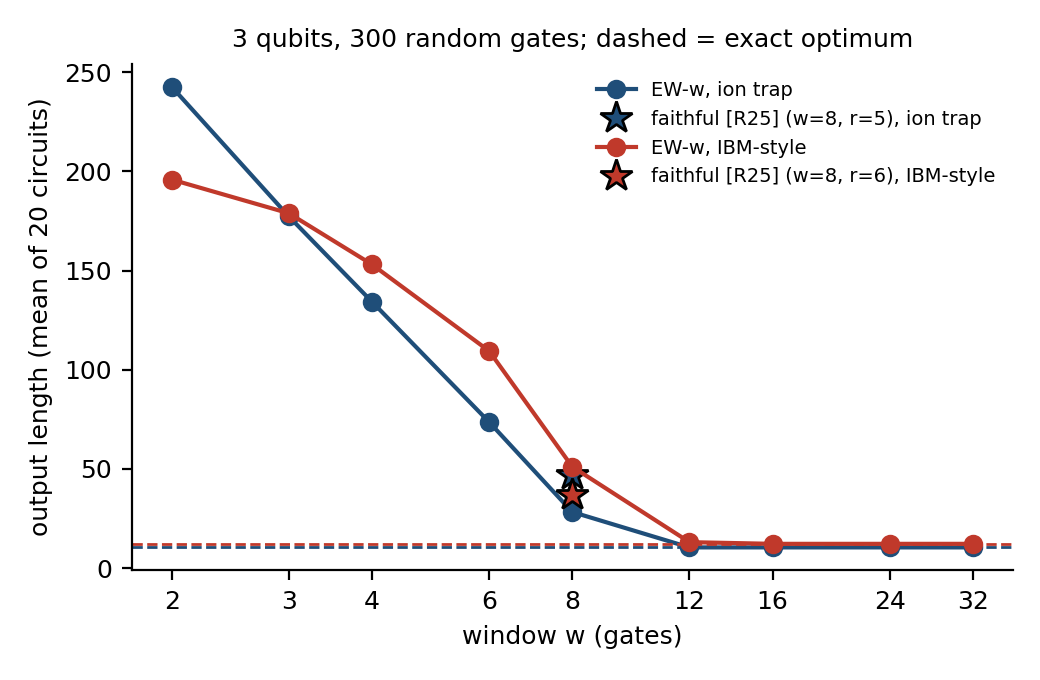
\includegraphics[width=0.49\textwidth]{figs/ext_window.png}\hfill
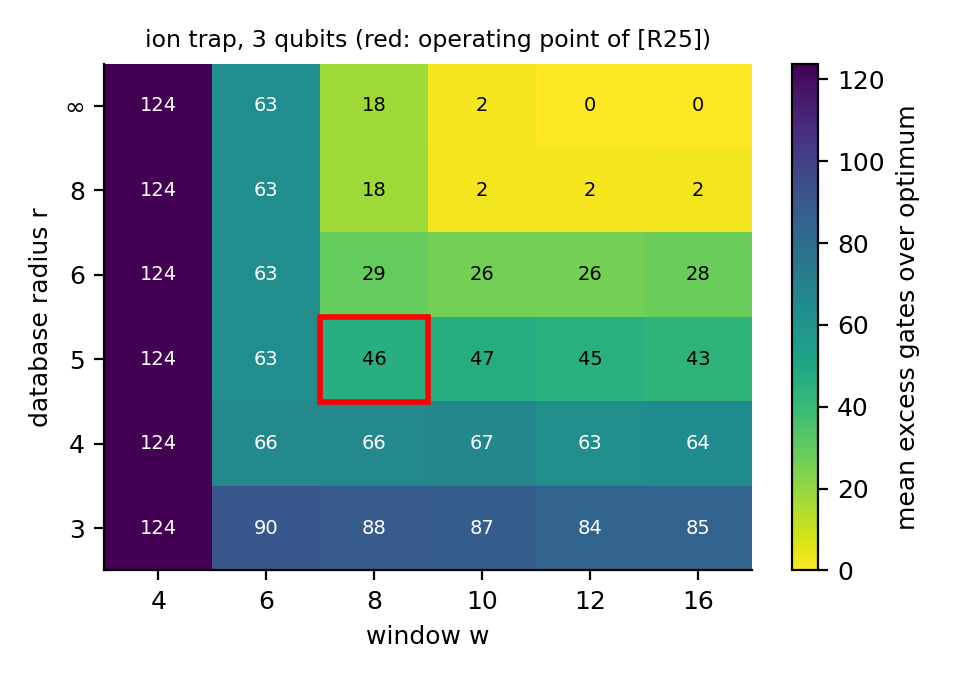
\includegraphics[width=0.49\textwidth]{figs/ext_grid.png}
\caption{Left, the fixed-point length of EW-$w$ against $w$, with the cascade transition near $w^\star$. Right, the mean excess
over the optimum by window $w$ and database radius $r$ (ion), with the original operating point $(8,5)$ marked.}\label{fig:window}\label{fig:grid}
\end{figure}

\clearpage

\begin{table}[h!]
\caption{Journal benchmark (4 qubits, 300 gates, 100 circuits). Original (orig.) and Qiskit level 3 use the first 30 circuits. Published (publ.)
numbers are from the journal version of~\cite{rosenhahn2025}. BQSKit level 4 is our run on the first \BqFourN\ circuits, with the
same gate set at continuous angles (approximate, all-to-all).}\label{tab:four}
\small\setlength{\tabcolsep}{3pt}
\begin{tabular*}{\textwidth}{@{\extracolsep\fill}lcccccccc}
\toprule
& bound & CW-sem & CW-24 & EW-16 & orig. & publ. & Qiskit & BQSKit\\
\midrule
ion, total & $\ge$\LBFourIon & \NjpIonCliff & \CWFourIon & \EWFourIon & \FaithFourIon & 111 & \QFourIon & \BqFourIon\\
ion, $\RXX$ & -- & -- & \CWFourIonTwoQ & \EWFourIonTwoQ & \FaithFourIonTwoQ & 43 & \QFourIonTwoQ & \BqFourIonTwoQ\\
IBM-style, total & $\ge$\LBFourIbm & \NjpIbmCliff & \CWFourIbm & \EWFourIbm & \FaithFourIbm & 107 & \QFourIbm & \BqFourIbm\\
IBM-style, $\CZ$ & -- & -- & \CWFourIbmTwoQ & \EWFourIbmTwoQ & \FaithFourIbmTwoQ & 43 & \QFourIbmTwoQ & \BqFourIbmTwoQ\\
\botrule
\end{tabular*}
\end{table}

\clearpage
\bibliography{refs}
\end{document}
